Para atestar o requisito de que o mecanismo deve funcionar em topologias genéricas independentemente do número de dispositivos, a rede triângulo original foi modificada. Criou-se um quarto nó (\texttt{Switch 4}) conectado em série ao \texttt{Switch 3}, permitindo validar saltos mais longos e rotas assimétricas.

\begin{figure}[H]
    \centering
    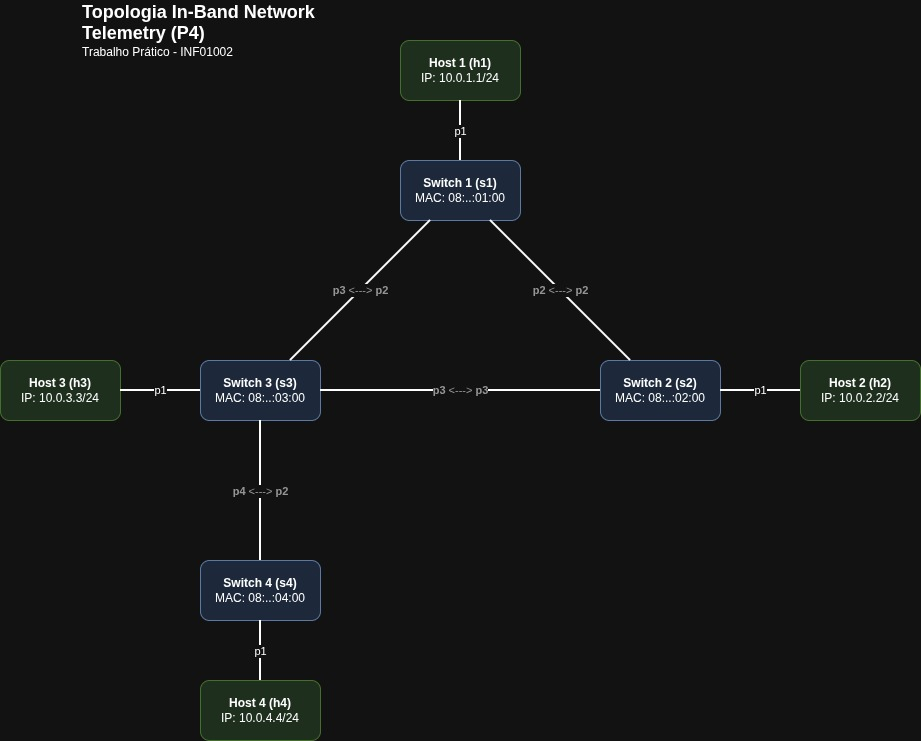
\includegraphics[width=0.8\textwidth]{figures/topologia_draw_io.jpg}
    \caption{Topologia da rede.}
\end{figure}

\begin{figure}[H]
    \centering
    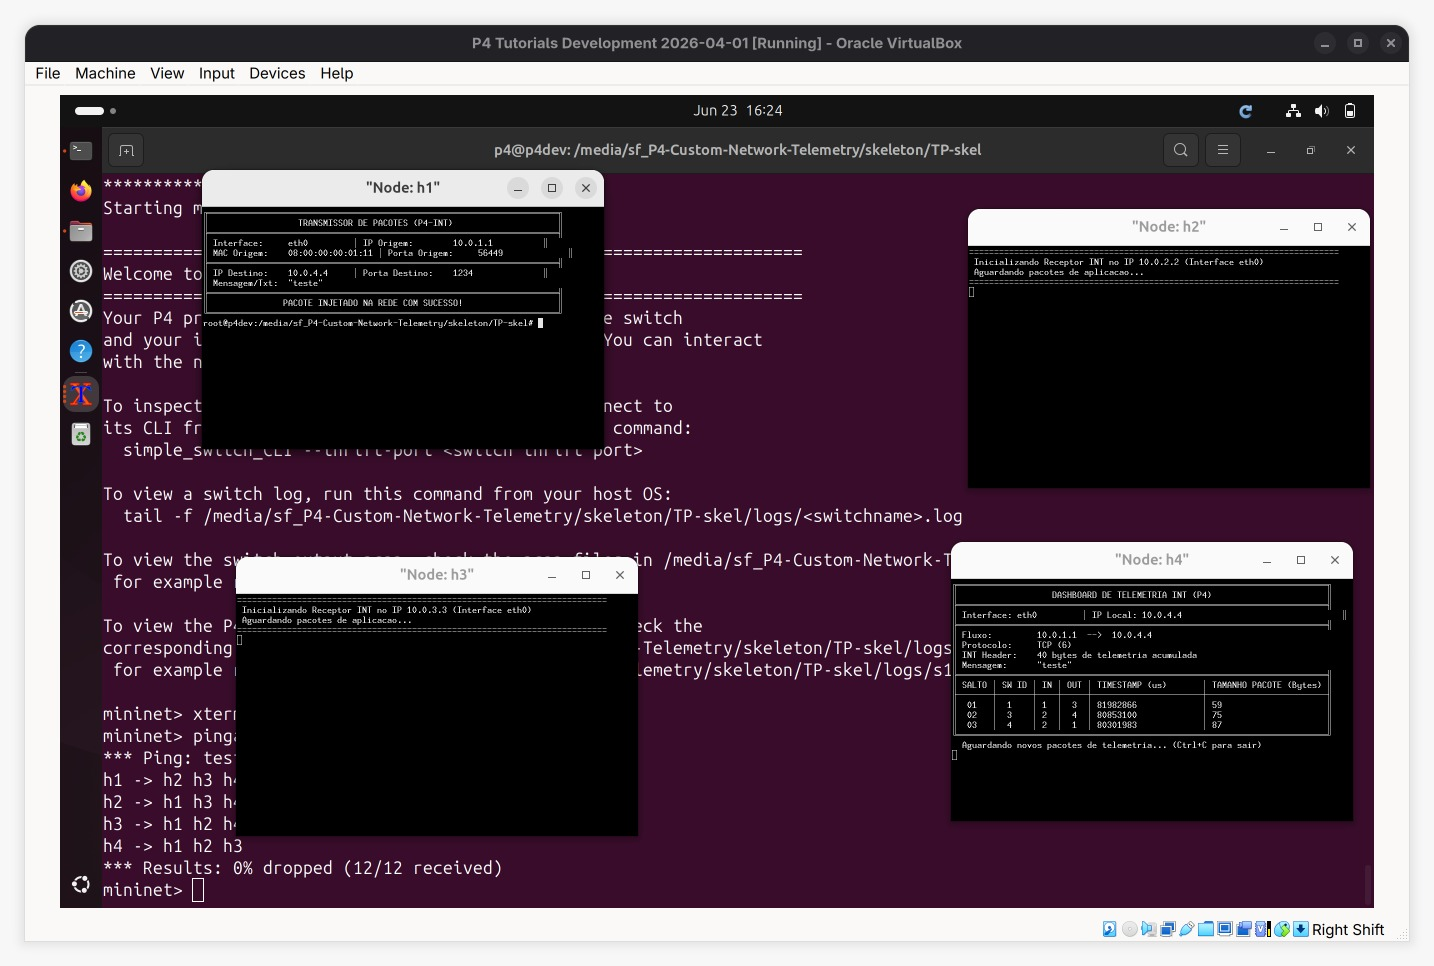
\includegraphics[width=0.8\textwidth]{figures/print.jpeg}
    \caption{Teste com 3 saltos.}
\end{figure}

Durante a extração dos dados na tabela TUI, observou-se que o \textit{timestamp} de um switch final no caminho pode apresentar valor inferior ao de um switch anterior. Esse comportamento comprova a natureza da simulação do BMv2 no Mininet, onde os processos não possuem sincronismo via \textit{Precision Time Protocol} (PTP), tornando os relógios independentes. Contudo, o acúmulo de saltos opera de forma contínua e robusta.
